\chapter{Question 2}
\label{avoiding-uri-aliases} 

\textbf{Write a Python program that:}

\begin{itemize}
\item\textbf{takes as a command line argument a web page}
\item\textbf{extracts all the links from the page}
\item \textbf{lists all the links that result in PDF files, and prints out the bytes for each of the links.  (note: be sure to follow  all the redirects until the link terminates with a ``200 OK''.)}
\item \textbf{show that the program works on 3 different URIs, one of which needs to be:{\url {http://www.cs.odu.edu/~mln/teaching/cs532-s16/test/pdfs.html}}} 
\end{itemize}
For solving the above problem I have written a program using Python. Following are the steps I've taken to solve the problem: 
\begin{itemize}
\item  The python script takes the web page as command line argument, finds all the links with ``a'' tag and passes its href to the function getsize().

\item This function fetches the content-length, content-type and status code for each link and extracts all the links that result in PDF files by checking if the content-type is ``application/pdf'' and if the status code is ``200''.

\item The output of the program prints the links that are PDF files and its size.
\end{itemize}
\newpage

\lstinputlisting[language=Python,caption=``Python code for extracting links that are PDF files'',frame=single,breaklines=true,captionpos=b,numbers=left,showspaces=false,showstringspaces=false,basicstyle=\footnotesize]{src/extractPDF.py}
\begin{itemize}
\item To run the code, go to the folder where the python code is located. Type {\color{blue} python extractPDF.py $<$link$>$} to see the output.
\item I tried to run the code for URIs which use relative path in the href, but my program wasn't returning any URI with PDFs as the href gets appended to the base URI. I did not handle this case. This can be handled by appending this relative href to the base URI.
\item I ran the program on three different URIs.
\end{itemize}

\begin{figure}[h!]
\begin{center}
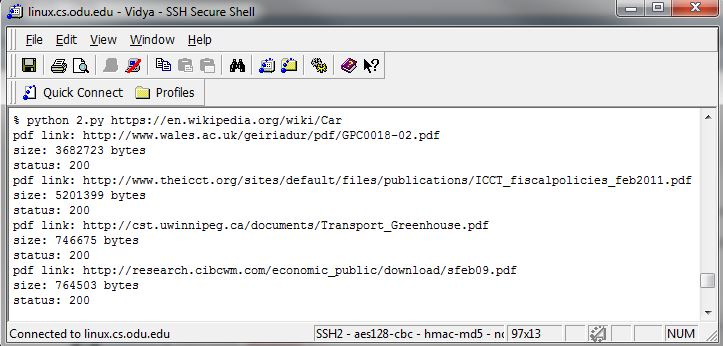
\includegraphics[scale=0.55, keepaspectratio=true]{figures/URI1.JPG}
\caption{Output for URI \url {https://en.wikipedia.org/wiki/Car}}
\label{mcpon_navy_mil}
\end{center}
\end{figure}


\begin{figure}[h!]
\begin{center}
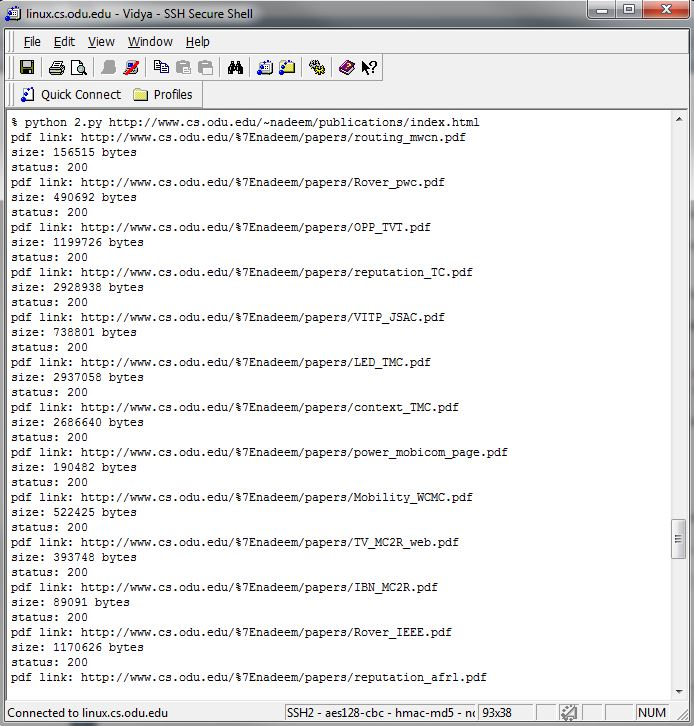
\includegraphics[scale=0.55, keepaspectratio=true]{figures/URI2.JPG}
\caption{Output for URI \url {http://www.cs.odu.edu/~nadeem/publications/index.html}}
\label{mcpon_navy_mil}
\end{center}
\end{figure}


\begin{figure}[h!]
\begin{center}
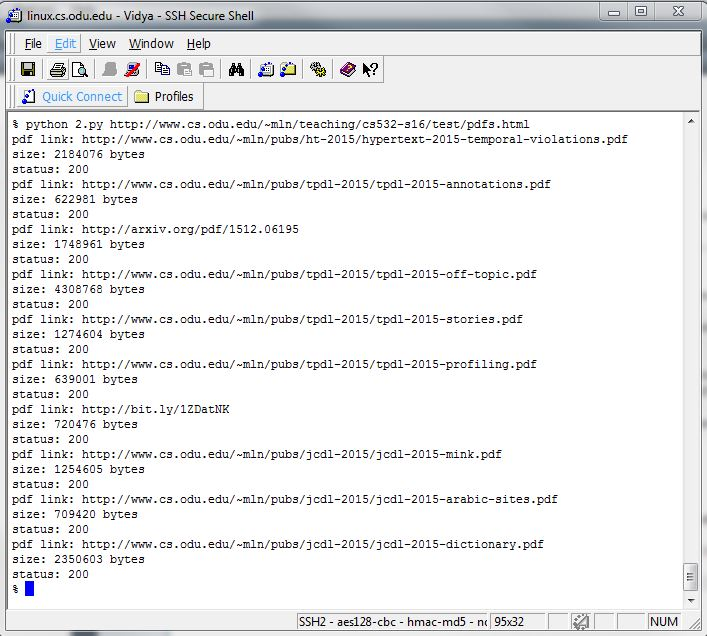
\includegraphics[scale=0.55, keepaspectratio=true]{figures/URI3.JPG}
\caption{Output for URI \url {http://www.cs.odu.edu/~mln/teaching/cs532-s16/test/pdfs.html}}
\label{mcpon_navy_mil}
\end{center}
\end{figure}